% GNUPLOT: LaTeX picture with Postscript
\begingroup
  \makeatletter
  \providecommand\color[2][]{%
    \GenericError{(gnuplot) \space\space\space\@spaces}{%
      Package color not loaded in conjunction with
      terminal option `colourtext'%
    }{See the gnuplot documentation for explanation.%
    }{Either use 'blacktext' in gnuplot or load the package
      color.sty in LaTeX.}%
    \renewcommand\color[2][]{}%
  }%
  \providecommand\includegraphics[2][]{%
    \GenericError{(gnuplot) \space\space\space\@spaces}{%
      Package graphicx or graphics not loaded%
    }{See the gnuplot documentation for explanation.%
    }{The gnuplot epslatex terminal needs graphicx.sty or graphics.sty.}%
    \renewcommand\includegraphics[2][]{}%
  }%
  \providecommand\rotatebox[2]{#2}%
  \@ifundefined{ifGPcolor}{%
    \newif\ifGPcolor
    \GPcolortrue
  }{}%
  \@ifundefined{ifGPblacktext}{%
    \newif\ifGPblacktext
    \GPblacktextfalse
  }{}%
  % define a \g@addto@macro without @ in the name:
  \let\gplgaddtomacro\g@addto@macro
  % define empty templates for all commands taking text:
  \gdef\gplbacktext{}%
  \gdef\gplfronttext{}%
  \makeatother
  \ifGPblacktext
    % no textcolor at all
    \def\colorrgb#1{}%
    \def\colorgray#1{}%
  \else
    % gray or color?
    \ifGPcolor
      \def\colorrgb#1{\color[rgb]{#1}}%
      \def\colorgray#1{\color[gray]{#1}}%
      \expandafter\def\csname LTw\endcsname{\color{white}}%
      \expandafter\def\csname LTb\endcsname{\color{black}}%
      \expandafter\def\csname LTa\endcsname{\color{black}}%
      \expandafter\def\csname LT0\endcsname{\color[rgb]{1,0,0}}%
      \expandafter\def\csname LT1\endcsname{\color[rgb]{0,1,0}}%
      \expandafter\def\csname LT2\endcsname{\color[rgb]{0,0,1}}%
      \expandafter\def\csname LT3\endcsname{\color[rgb]{1,0,1}}%
      \expandafter\def\csname LT4\endcsname{\color[rgb]{0,1,1}}%
      \expandafter\def\csname LT5\endcsname{\color[rgb]{1,1,0}}%
      \expandafter\def\csname LT6\endcsname{\color[rgb]{0,0,0}}%
      \expandafter\def\csname LT7\endcsname{\color[rgb]{1,0.3,0}}%
      \expandafter\def\csname LT8\endcsname{\color[rgb]{0.5,0.5,0.5}}%
    \else
      % gray
      \def\colorrgb#1{\color{black}}%
      \def\colorgray#1{\color[gray]{#1}}%
      \expandafter\def\csname LTw\endcsname{\color{white}}%
      \expandafter\def\csname LTb\endcsname{\color{black}}%
      \expandafter\def\csname LTa\endcsname{\color{black}}%
      \expandafter\def\csname LT0\endcsname{\color{black}}%
      \expandafter\def\csname LT1\endcsname{\color{black}}%
      \expandafter\def\csname LT2\endcsname{\color{black}}%
      \expandafter\def\csname LT3\endcsname{\color{black}}%
      \expandafter\def\csname LT4\endcsname{\color{black}}%
      \expandafter\def\csname LT5\endcsname{\color{black}}%
      \expandafter\def\csname LT6\endcsname{\color{black}}%
      \expandafter\def\csname LT7\endcsname{\color{black}}%
      \expandafter\def\csname LT8\endcsname{\color{black}}%
    \fi
  \fi
    \setlength{\unitlength}{0.0500bp}%
    \ifx\gptboxheight\undefined%
      \newlength{\gptboxheight}%
      \newlength{\gptboxwidth}%
      \newsavebox{\gptboxtext}%
    \fi%
    \setlength{\fboxrule}{0.5pt}%
    \setlength{\fboxsep}{1pt}%
\begin{picture}(10080.00,3772.00)%
    \gplgaddtomacro\gplbacktext{%
      \csname LTb\endcsname%
      \put(396,594){\makebox(0,0)[r]{\strut{}\footnotesize{$-0.8$}}}%
      \csname LTb\endcsname%
      \put(396,909){\makebox(0,0)[r]{\strut{}\footnotesize{$-0.6$}}}%
      \csname LTb\endcsname%
      \put(396,1223){\makebox(0,0)[r]{\strut{}\footnotesize{$-0.4$}}}%
      \csname LTb\endcsname%
      \put(396,1538){\makebox(0,0)[r]{\strut{}\footnotesize{$-0.2$}}}%
      \csname LTb\endcsname%
      \put(396,1853){\makebox(0,0)[r]{\strut{}\footnotesize{$0$}}}%
      \csname LTb\endcsname%
      \put(396,2167){\makebox(0,0)[r]{\strut{}\footnotesize{$0.2$}}}%
      \csname LTb\endcsname%
      \put(396,2482){\makebox(0,0)[r]{\strut{}\footnotesize{$0.4$}}}%
      \csname LTb\endcsname%
      \put(396,2796){\makebox(0,0)[r]{\strut{}\footnotesize{$0.6$}}}%
      \csname LTb\endcsname%
      \put(396,3111){\makebox(0,0)[r]{\strut{}\footnotesize{$0.8$}}}%
      \csname LTb\endcsname%
      \put(528,374){\makebox(0,0){\strut{}\footnotesize{$0$}}}%
      \csname LTb\endcsname%
      \put(1026,374){\makebox(0,0){\strut{}\footnotesize{$8$}}}%
      \csname LTb\endcsname%
      \put(1524,374){\makebox(0,0){\strut{}\footnotesize{$16$}}}%
      \csname LTb\endcsname%
      \put(2022,374){\makebox(0,0){\strut{}\footnotesize{$24$}}}%
      \csname LTb\endcsname%
      \put(2520,374){\makebox(0,0){\strut{}\footnotesize{$32$}}}%
      \csname LTb\endcsname%
      \put(3017,374){\makebox(0,0){\strut{}\footnotesize{$40$}}}%
      \csname LTb\endcsname%
      \put(3515,374){\makebox(0,0){\strut{}\footnotesize{$48$}}}%
      \csname LTb\endcsname%
      \put(4013,374){\makebox(0,0){\strut{}\footnotesize{$56$}}}%
      \csname LTb\endcsname%
      \put(4511,374){\makebox(0,0){\strut{}\footnotesize{$64$}}}%
    }%
    \gplgaddtomacro\gplfronttext{%
      \csname LTb\endcsname%
      \put(-176,1852){\rotatebox{-270}{\makebox(0,0){\strut{}\footnotesize{$cos(2\pi fi)$}}}}%
      \put(2519,154){\makebox(0,0){\strut{}\footnotesize{$i$}}}%
      \put(2519,3441){\makebox(0,0){\strut{}\shortstack{input\\ $N=64$ $f=0.1$ $dB=-5$}}}%
    }%
    \gplgaddtomacro\gplbacktext{%
      \csname LTb\endcsname%
      \put(5436,594){\makebox(0,0)[r]{\strut{}\footnotesize{$10^{-5}$}}}%
      \csname LTb\endcsname%
      \put(5436,1014){\makebox(0,0)[r]{\strut{}\footnotesize{$10^{-4}$}}}%
      \csname LTb\endcsname%
      \put(5436,1433){\makebox(0,0)[r]{\strut{}\footnotesize{$10^{-3}$}}}%
      \csname LTb\endcsname%
      \put(5436,1853){\makebox(0,0)[r]{\strut{}\footnotesize{$10^{-2}$}}}%
      \csname LTb\endcsname%
      \put(5436,2272){\makebox(0,0)[r]{\strut{}\footnotesize{$10^{-1}$}}}%
      \csname LTb\endcsname%
      \put(5436,2692){\makebox(0,0)[r]{\strut{}\footnotesize{$10^{0}$}}}%
      \csname LTb\endcsname%
      \put(5436,3111){\makebox(0,0)[r]{\strut{}\footnotesize{$10^{1}$}}}%
      \csname LTb\endcsname%
      \put(5568,374){\makebox(0,0){\strut{}\footnotesize{$0$}}}%
      \csname LTb\endcsname%
      \put(6066,374){\makebox(0,0){\strut{}\footnotesize{$8$}}}%
      \csname LTb\endcsname%
      \put(6564,374){\makebox(0,0){\strut{}\footnotesize{$16$}}}%
      \csname LTb\endcsname%
      \put(7062,374){\makebox(0,0){\strut{}\footnotesize{$24$}}}%
      \csname LTb\endcsname%
      \put(7560,374){\makebox(0,0){\strut{}\footnotesize{$32$}}}%
      \csname LTb\endcsname%
      \put(8057,374){\makebox(0,0){\strut{}\footnotesize{$40$}}}%
      \csname LTb\endcsname%
      \put(8555,374){\makebox(0,0){\strut{}\footnotesize{$48$}}}%
      \csname LTb\endcsname%
      \put(9053,374){\makebox(0,0){\strut{}\footnotesize{$56$}}}%
      \csname LTb\endcsname%
      \put(9551,374){\makebox(0,0){\strut{}\footnotesize{$64$}}}%
    }%
    \gplgaddtomacro\gplfronttext{%
      \csname LTb\endcsname%
      \put(4864,1852){\rotatebox{-270}{\makebox(0,0){\strut{}\footnotesize{$|X_n|$}}}}%
      \put(7559,154){\makebox(0,0){\strut{}\footnotesize{$n$}}}%
      \put(7559,3441){\makebox(0,0){\strut{}\shortstack{FFT\\ $N=64$ $f=0.1$ $dB=-5$}}}%
      \csname LTb\endcsname%
      \put(6934,2938){\makebox(0,0)[l]{\strut{}\tiny{FFT64 FP}}}%
      \csname LTb\endcsname%
      \put(6934,2718){\makebox(0,0)[l]{\strut{}\tiny{FFT64 Q1.15 }}}%
      \csname LTb\endcsname%
      \put(6934,2498){\makebox(0,0)[l]{\strut{}\tiny{FFT64 Q11.15}}}%
    }%
    \gplbacktext
    \put(0,0){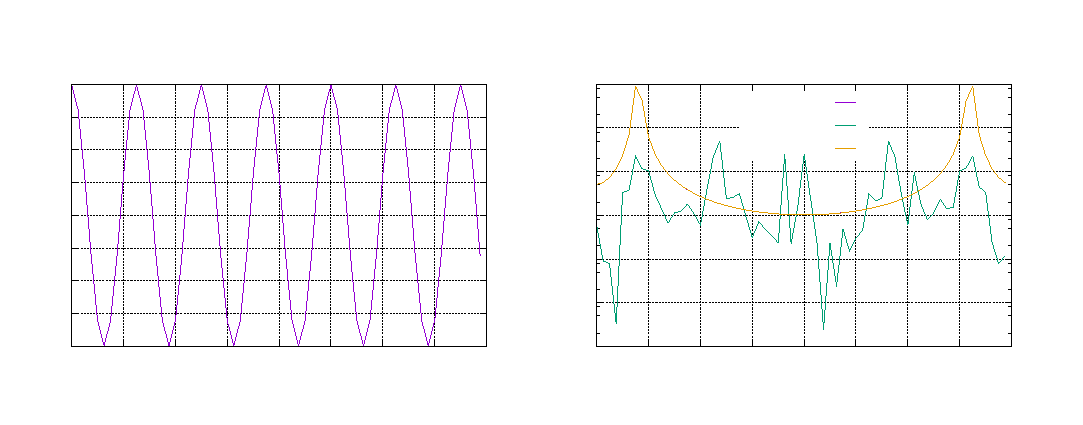
\includegraphics{cosineFFT}}%
    \gplfronttext
  \end{picture}%
\endgroup
